\documentclass[journal,12pt,twocolumn]{IEEEtran}
\usepackage{setspace}
\usepackage{gensymb}
\usepackage{caption}
%\usepackage{multirow}
%\usepackage{multicolumn}
%\usepackage{subcaption}
%\doublespacing
\singlespacing
\usepackage{csvsimple}
\usepackage{amsmath}
\usepackage{multicol}
%\usepackage{enumerate}
\usepackage{amssymb}
%\usepackage{graphicx}
\usepackage{newfloat}
%\usepackage{syntax}
\usepackage{listings}
\usepackage{iithtlc}
\usepackage{color}
\usepackage{tikz}
\usetikzlibrary{shapes,arrows}



%\usepackage{graphicx}
%\usepackage{amssymb}
%\usepackage{relsize}
%\usepackage[cmex10]{amsmath}
%\usepackage{mathtools}
%\usepackage{amsthm}
%\interdisplaylinepenalty=2500
%\savesymbol{iint}
%\usepackage{txfonts}
%\restoresymbol{TXF}{iint}
%\usepackage{wasysym}
\usepackage{amsthm}
\usepackage{mathrsfs}
\usepackage{txfonts}
\usepackage{stfloats}
\usepackage{cite}
\usepackage{cases}
\usepackage{mathtools}
\usepackage{caption}
\usepackage{enumerate}	
\usepackage{enumitem}
\usepackage{amsmath}
%\usepackage{xtab}
\usepackage{longtable}
\usepackage{multirow}
%\usepackage{algorithm}
%\usepackage{algpseudocode}
\usepackage{enumitem}
\usepackage{mathtools}
\usepackage{hyperref}
%\usepackage[framemethod=tikz]{mdframed}
\usepackage{listings}
    %\usepackage[latin1]{inputenc}                                 %%
    \usepackage{color}                                            %%
    \usepackage{array}                                            %%
    \usepackage{longtable}                                        %%
    \usepackage{calc}                                             %%
    \usepackage{multirow}                                         %%
    \usepackage{hhline}                                           %%
    \usepackage{ifthen}                                           %%
  %optionally (for landscape tables embedded in another document): %%
    \usepackage{lscape}     


\usepackage{url}
\def\UrlBreaks{\do\/\do-}


%\usepackage{stmaryrd}


%\usepackage{wasysym}
%\newcounter{MYtempeqncnt}
\DeclareMathOperator*{\Res}{Res}
%\renewcommand{\baselinestretch}{2}
\renewcommand\thesection{\arabic{section}}
\renewcommand\thesubsection{\thesection.\arabic{subsection}}
\renewcommand\thesubsubsection{\thesubsection.\arabic{subsubsection}}

\renewcommand\thesectiondis{\arabic{section}}
\renewcommand\thesubsectiondis{\thesectiondis.\arabic{subsection}}
\renewcommand\thesubsubsectiondis{\thesubsectiondis.\arabic{subsubsection}}

% correct bad hyphenation here
\hyphenation{op-tical net-works semi-conduc-tor}

%\lstset{
%language=C,
%frame=single, 
%breaklines=true
%}

%\lstset{
	%%basicstyle=\small\ttfamily\bfseries,
	%%numberstyle=\small\ttfamily,
	%language=Octave,
	%backgroundcolor=\color{white},
	%%frame=single,
	%%keywordstyle=\bfseries,
	%%breaklines=true,
	%%showstringspaces=false,
	%%xleftmargin=-10mm,
	%%aboveskip=-1mm,
	%%belowskip=0mm
%}

%\surroundwithmdframed[width=\columnwidth]{lstlisting}
\def\inputGnumericTable{}                                 %%
\lstset{
%language=C,
frame=single, 
breaklines=true,
columns=fullflexible
}
 

\begin{document}
%
\tikzstyle{block} = [rectangle, draw,
    text width=3em, text centered, minimum height=3em]
\tikzstyle{sum} = [draw, circle, node distance=3cm]
\tikzstyle{input} = [coordinate]
\tikzstyle{output} = [coordinate]
\tikzstyle{pinstyle} = [pin edge={to-,thin,black}]

\theoremstyle{definition}
\newtheorem{theorem}{Theorem}[section]
\newtheorem{problem}{Problem}
\newtheorem{proposition}{Proposition}[section]
\newtheorem{lemma}{Lemma}[section]
\newtheorem{corollary}[theorem]{Corollary}
\newtheorem{example}{Example}[section]
\newtheorem{definition}{Definition}[section]
%\newtheorem{algorithm}{Algorithm}[section]
%\newtheorem{cor}{Corollary}
\newcommand{\BEQA}{\begin{eqnarray}}
\newcommand{\EEQA}{\end{eqnarray}}
\newcommand{\define}{\stackrel{\triangle}{=}}

\bibliographystyle{IEEEtran}
%\bibliographystyle{ieeetr}

\providecommand{\nCr}[2]{\,^{#1}C_{#2}} % nCr
\providecommand{\nPr}[2]{\,^{#1}P_{#2}} % nPr
\providecommand{\mbf}{\mathbf}
\providecommand{\pr}[1]{\ensuremath{\Pr\left(#1\right)}}
\providecommand{\qfunc}[1]{\ensuremath{Q\left(#1\right)}}
\providecommand{\sbrak}[1]{\ensuremath{{}\left[#1\right]}}
\providecommand{\lsbrak}[1]{\ensuremath{{}\left[#1\right.}}
\providecommand{\rsbrak}[1]{\ensuremath{{}\left.#1\right]}}
\providecommand{\brak}[1]{\ensuremath{\left(#1\right)}}
\providecommand{\lbrak}[1]{\ensuremath{\left(#1\right.}}
\providecommand{\rbrak}[1]{\ensuremath{\left.#1\right)}}
\providecommand{\cbrak}[1]{\ensuremath{\left\{#1\right\}}}
\providecommand{\lcbrak}[1]{\ensuremath{\left\{#1\right.}}
\providecommand{\rcbrak}[1]{\ensuremath{\left.#1\right\}}}
\theoremstyle{remark}
\newtheorem{rem}{Remark}
\newcommand{\sgn}{\mathop{\mathrm{sgn}}}
\providecommand{\abs}[1]{\left\vert#1\right\vert}
\providecommand{\res}[1]{\Res\displaylimits_{#1}} 
\providecommand{\norm}[1]{\lVert#1\rVert}
\providecommand{\mtx}[1]{\mathbf{#1}}
\providecommand{\mean}[1]{E\left[ #1 \right]}
\providecommand{\fourier}{\overset{\mathcal{F}}{ \rightleftharpoons}}
%\providecommand{\hilbert}{\overset{\mathcal{H}}{ \rightleftharpoons}}
\providecommand{\system}{\overset{\mathcal{H}}{ \longleftrightarrow}}
	%\newcommand{\solution}[2]{\textbf{Solution:}{#1}}
\newcommand{\solution}{\noindent \textbf{Solution: }}
\newcommand{\myvec}[1]{\ensuremath{\begin{pmatrix}#1\end{pmatrix}}}
\providecommand{\dec}[2]{\ensuremath{\overset{#1}{\underset{#2}{\gtrless}}}}
\DeclarePairedDelimiter{\ceil}{\lceil}{\rceil}
%\numberwithin{equation}{subsection}
\numberwithin{equation}{section}
%\numberwithin{problem}{subsection}
%\numberwithin{definition}{subsection}
\makeatletter
\@addtoreset{figure}{section}
\makeatother

\let\StandardTheFigure\thefigure
%\renewcommand{\thefigure}{\theproblem.\arabic{figure}}
\renewcommand{\thefigure}{\thesection}


%\numberwithin{figure}{subsection}

%\numberwithin{equation}{subsection}
%\numberwithin{equation}{section}
%\numberwithin{equation}{problem}
%\numberwithin{problem}{subsection}
\numberwithin{problem}{section}
%%\numberwithin{definition}{subsection}
%\makeatletter
%\@addtoreset{figure}{problem}
%\makeatother
\makeatletter
\@addtoreset{table}{section}
\makeatother

\let\StandardTheFigure\thefigure
\let\StandardTheTable\thetable
\let\vec\mathbf
%%\renewcommand{\thefigure}{\theproblem.\arabic{figure}}
%\renewcommand{\thefigure}{\theproblem}

%%\numberwithin{figure}{section}

%%\numberwithin{figure}{subsection}



\def\putbox#1#2#3{\makebox[0in][l]{\makebox[#1][l]{}\raisebox{\baselineskip}[0in][0in]{\raisebox{#2}[0in][0in]{#3}}}}
     \def\rightbox#1{\makebox[0in][r]{#1}}
     \def\centbox#1{\makebox[0in]{#1}}
     \def\topbox#1{\raisebox{-\baselineskip}[0in][0in]{#1}}
     \def\midbox#1{\raisebox{-0.5\baselineskip}[0in][0in]{#1}}

\vspace{3cm}

\title{ 
	\logo{
Linear Algebra through Coordinate Geometry 
	}
}

\author{ G V V Sharma$^{*}$% <-this % stops a space
	\thanks{*The author is with the Department
		of Electrical Engineering, Indian Institute of Technology, Hyderabad
		502285 India e-mail:  gadepall@iith.ac.in. All content in this manual is released under GNU GPL.  Free and open source.}
	
}	

\maketitle

\tableofcontents

\bigskip

\renewcommand{\thefigure}{\theenumi}
\renewcommand{\thetable}{\theenumi}


\begin{abstract}
	
This manual introduces linear algebra through coordinate geometry using a problem solving approach.
\end{abstract}
\section{The Straight Line}
\begin{enumerate}[label=\thesection.\arabic*
,ref=\thesection.\theenumi]
\item The equation of the line between two points $\vec{A}$ and $\vec{B}$ is given by
\begin{equation}
\vec{x} = \vec{A} + \lambda \brak{\vec{A}-\vec{B}}
\end{equation}
%
Alternatively, it can be expressed as
\begin{equation}
\label{eq:line_normal}
\vec{m}^T\brak{\vec{x}-\vec{A}} = 0
\end{equation}
%
where $\vec{m}$ is the solution of
\begin{equation}
\label{eq:normal_slope}
\brak{\vec{A}-\vec{B}}^T\vec{m} = 0
\end{equation}
\item The line through
\begin{equation}
\label{eq:locus}
\vec{A}=\myvec{2\\3}
\end{equation}
intersects the coordinate axes at $\vec{P}$ and $\vec{Q}$. If $\vec{O}$ is the origin and rectangle $OPRQ$ is 
completed, find the locus of $\vec{R}$.
\begin{figure}
\centering
\includegraphics[width=\columnwidth]{./figs/locus.eps}
\caption{}
\label{fig:locus}
\end{figure}
\\
\solution From Fig. \eqref{fig:locus},
\begin{align}
\vec{P}&= \myvec{1 & 0\\ 0 & 0}\vec{R}
\label{eq:locusp}
\\
\vec{Q}&= \myvec{0 & 0\\ 0 & 1}\vec{R}
\label{eq:locusq}
\\
\vec{P}+\vec{Q} &=\vec{R}
\label{eq:locusr}
\end{align}
From \eqref{eq:line_normal} and \eqref{eq:normal_slope},
\begin{align}
\begin{split}
\brak{\vec{A}-\vec{P}}^T\vec{m} &= 0
\\
\brak{\vec{A}-\vec{Q}}^T\vec{m} &= 0
\\
\brak{\vec{P}-\vec{Q}}^T\vec{m} &= 0
\end{split}
\label{eq:locus_apq}
\end{align}
%
From \eqref{eq:locus_apq} and \eqref{eq:locus_ar}
\begin{align}
\sbrak{\vec{2A}-\brak{\vec{P}+\vec{Q}}}^T\vec{m} &= 0
\\
\implies \brak{\vec{2A}-\vec{R}}^T\vec{m} &= 0
\end{align}
%
From \eqref{eq:locus_apq} and \eqref{eq:locusp},\eqref{eq:locusq}

%\\
%\implies 
%\frac{\vec{P}- \myvec{2 \\ 3}}{\lambda_1}
%&=
%\frac{\vec{Q}-\myvec{2 \\ 3}}{ \lambda_2}
%\\
%\implies \vec{P} - k\vec{Q} &= \brak{1-k}\myvec{2 \\ 3}
%\\
%\implies \myvec{\vec{P} & \vec{Q} }\myvec{1 \\ - k}
% &= \brak{1-k}\myvec{2 \\ 3}
%\label{eq:locus_one}
Also,
\begin{align}
\vec{P}+\vec{Q}&= \vec{R}
\\
\implies \myvec{\vec{P} & \vec{Q} }\myvec{1 \\ 1} &= \vec{R}
\label{eq:locus_two}
\end{align}
%
From \eqref{eq:locus_one} and \eqref{eq:locus_two}
%
\begin{align}
\myvec{\vec{P} & \vec{Q} }\myvec{1 & 1  \\ 1 & -k} &= \myvec{\vec{R} & \brak{1-k}\myvec{2 \\ 3}}
\label{eq:locus_two}
\end{align}

\begin{align}
\implies \frac{\myvec{1 & 0 \\ 0 & 0}\vec{R} -  \myvec{2 \\ 3}}{ \lambda_1 } &= \frac{\myvec{0 & 0 \\ 0 & 
1}\vec{R} -  \myvec{2 \\ 3}}{ \lambda_2 }
\\
\implies \myvec{1 & 0 \\ 0 & -k}\vec{R}  &= \brak{1-k}  \myvec{2 \\ 3}
\end{align}

Let $\vec{x}=\myvec{x_1\\x_2}$ be any point on $OA$.
Then, using similar triangles,
\begin{align}
\frac{x_2}{x_1} &= \frac{a_2}{a_1} = m
\\
\implies x_2 &=  m x_1
\end{align}
where $m$ is known as the slope of the line. Thus, the equation of the line is
\begin{align}
%\label{eq:homog}
\vec{x} = \myvec{x_1\\m x_1} = x_1 \myvec{1 \\ m}
\end{align}
In general, the above equation is written as
\begin{align}
\label{eq:homog}
\vec{x} = \myvec{x_1\\m x_1} = \lambda \myvec{1 \\ m}
\end{align}


\item Find the equation of $AB$ in Fig. \ref{fig:line_nhomog}
\begin{figure}
\centering
\includegraphics[width=\columnwidth]{./figs/line_nhomog.eps}
\caption{}
\label{fig:line_nhomog}
\end{figure}
\\
\solution 
From Fig. \ref{fig:line_nhomog}, 
%
\begin{align}
\frac{x_2-a_2}{x_1-a_1} = \frac{b_2-a_2}{b_1-a_1} = m
\\
\implies x_2 = m x_1 + a_2-ma_1
\label{eq:line_shift}
\end{align}
%
From \eqref{eq:line_shift},
\begin{align}
\myvec{x_1 \\ x_2} &= 
\myvec{x_1 \\   m x_1 + a_2-ma_1
} 
\\
&=\vec{A} + \brak{x_1-a_1}  \myvec{1 \\ m}
\\
&=\vec{A} + \lambda  \myvec{1 \\ m}
\label{eq:nhomog}
\end{align}

\item Find the length of $\vec{A}$ in Fig. \ref{fig:line_homog}
\\
\solution Using Baudhayana's theorem, the length of the vector $\vec{A}$ is defined as
\begin{equation}
 \norm{\vec{A}} = OA = \sqrt{a_1^2 + a_2^2}
=\sqrt{\vec{A}^T\vec{A}}.
\end{equation}
%
Also, from \eqref{eq:homog}, 
\begin{equation}
\norm{\vec{A}} = \lambda \sqrt{1+m^2}
\end{equation}
%
Note that $\lambda$ is the variable that determines the length of $\vec{A}$, 
since $m$ is constant for all points on the line.
%
\item Find $\vec{A}-\vec{B}$.
\begin{figure}
\centering
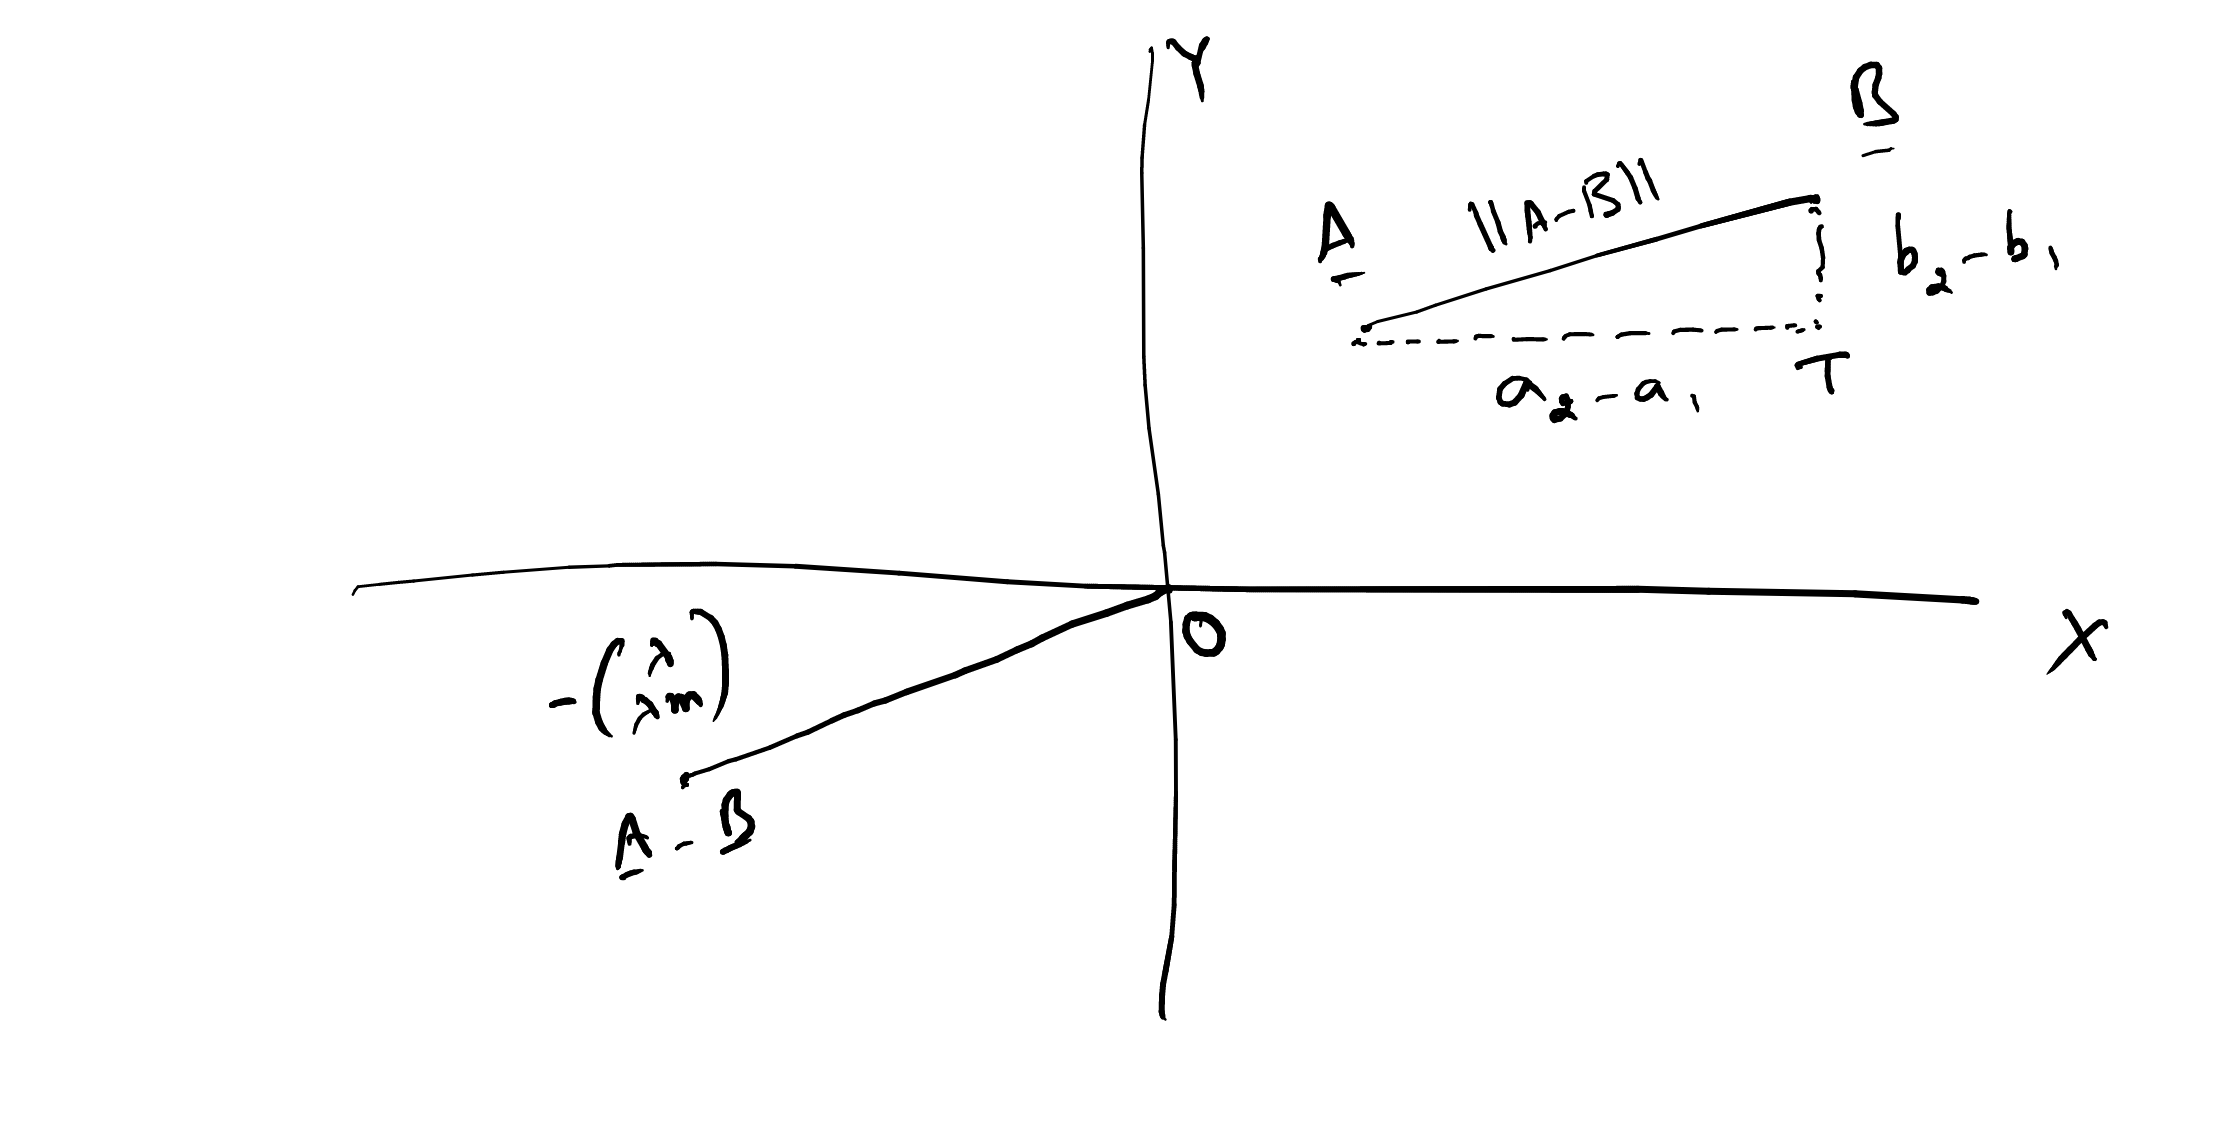
\includegraphics[width=\columnwidth]{./figs/ab.eps}
\caption{}
\label{fig:ab}
\end{figure}
%
\\
\solution See Fig. \ref{fig:ab}. From \eqref{eq:nhomog}, for some 
$\lambda$,
\begin{align}
\vec{B} &=\vec{A} + \lambda \myvec{1 \\ m}
\\
\implies \vec{A} - \vec{B} &= - \lambda \myvec{1 \\ m},
\end{align}
%
$\vec{A} - \vec{B}$ is marked in Fig. \ref{fig:ab}.
%
\item Show that $AB = \norm{\vec{A}-\vec{B}}$
\end{enumerate}
%
\section{Orthogonality}
\begin{enumerate}[label=\thesection.\arabic*
,ref=\thesection.\theenumi]
\item See Fig. \ref{fig:orth}.  In $\triangle ABC, AB \perp BC$. Show that
\begin{equation}
\brak{\vec{A}-\vec{B}}^T\brak{\vec{B}-\vec{C}} = 0
\label{eq:orth}
\end{equation}
\begin{figure}
\centering
\includegraphics[width=\columnwidth]{./figs/orth.eps}
\caption{}
\label{fig:orth}
\end{figure}
%
\solution Using Baudhayana's theorem,
\begin{align}
\norm{\vec{A}-\vec{B}}^2 + \norm{\vec{B}-\vec{C}}^2 &= 
\norm{\vec{C}-\vec{A}}^2
\\
\implies 
\brak{\vec{A}-\vec{B}}^T\brak{\vec{A}-\vec{B}} 
&+ 
\brak{\vec{B}-\vec{C}}^T\brak{\vec{B}-\vec{C}} 
\nonumber \\
&= 
\brak{\vec{C}-\vec{A}}^T \brak{\vec{C}-\vec{A}}
\nonumber \\
\implies 
2\vec{A}^T\vec{B} - 2\vec{B}^T\vec{B}&+2\vec{B}^T\vec{C}-2\vec{A}^T\vec{C}
=0
\end{align}
which can be simplified to obtain \eqref{eq:orth}.
%
\item Let $\vec{x}$ be any point on $AB$ in Fi.g \ref{fig:orth}.  Show that
\begin{equation}
\brak{\vec{x}-\vec{A}}^T\brak{\vec{B}-\vec{C}} = 0
\end{equation}
%
\item If $\vec{x,y}$ are any two points on $AB$, show that 
\begin{equation}
\label{eq:orth_any}
\brak{\vec{x}-\vec{y}}^T\brak{\vec{B}-\vec{C}} = 0
\end{equation}
%
\item In Fig. \ref{fig:alt}, $BE \perp AC, CF \perp AB$.  Show that $AD \perp BC$.
\begin{figure}[!hb]
\centering
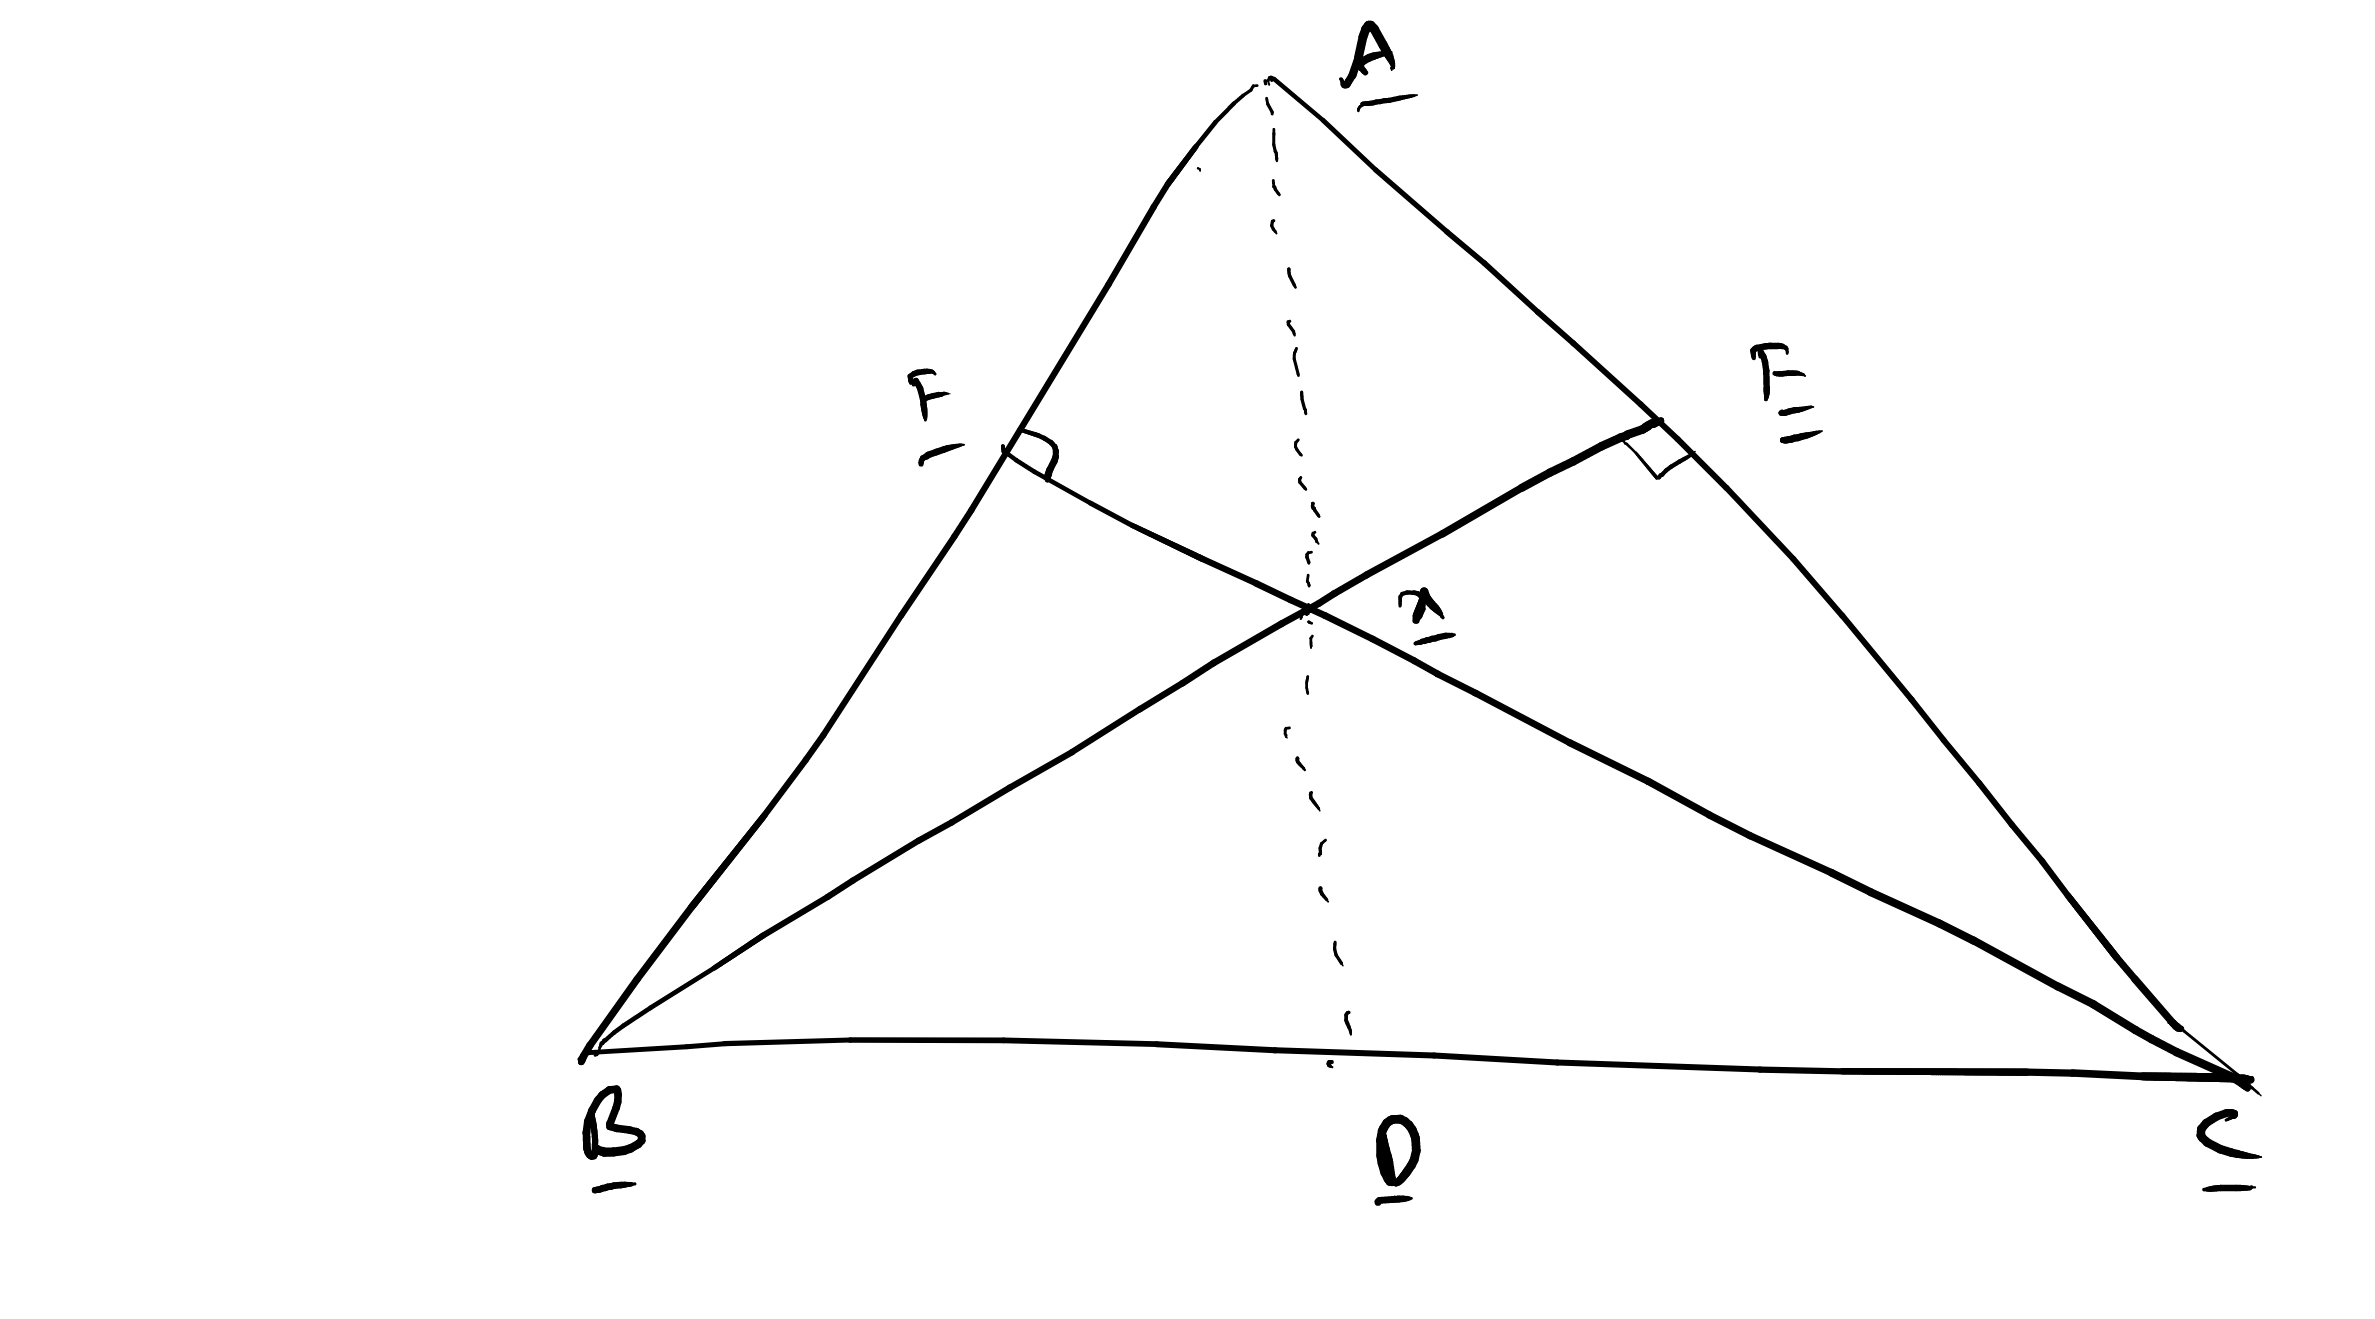
\includegraphics[width=\columnwidth]{./figs/alt.eps}
\caption{}
\label{fig:alt}
\end{figure}
\\
\solution Let $\vec{x}$ be the intersection of $BE$ and $CF$. Then, using 
\eqref{eq:orth_any},
\begin{align}
\label{eq:alt_1}
\begin{split}
\brak{\vec{x}-\vec{B}}^T
\brak{\vec{A}-\vec{C}} &= 0
\\
\brak{\vec{x}-\vec{C}}^T
\brak{\vec{A}-\vec{B}} &=0
\end{split}
\\
\label{eq:alt_3}
\implies \vec{x}^T\brak{\vec{A}-\vec{C}}-\vec{B}^T\brak{\vec{A}-\vec{C}} &= 0
\\
\text{and }\vec{x}^T\brak{\vec{A}-\vec{B}}-\vec{C}^T\brak{\vec{A}-\vec{B}} &= 0
\label{eq:alt_4}
\end{align}
%
Subtracting \eqref{eq:alt_4} from \eqref{eq:alt_3},
\begin{align}
\vec{x}^T\brak{\vec{B}-\vec{C}} + \vec{A}^T\brak{\vec{C}-\vec{B}} &= 0
\\
\implies \brak{\vec{x}^T - \vec{A}^T}\brak{\vec{B}-\vec{C}}  &= 0
\\
\implies \brak{\vec{x} - \vec{A}}^T\brak{\vec{B}-\vec{C}}  &= 0
\end{align}
%
which completes the proof.
\end{enumerate}
%
\section{Medians of a triangle}
\begin{enumerate}[label=\thesection.\arabic*
,ref=\thesection.\theenumi]
\item In Fig. \ref{fig:ratio},
\begin{equation}
\frac{AB}{BC} = \frac{\norm{\vec{A}-\vec{B}}}{\norm{\vec{B}-\vec{C}}} = k.
\label{eq:k}
\end{equation}
%
Show that
%
\begin{equation}
\frac{\vec{A}+k\vec{C}}{k+1} = \vec{B}.
\label{eq:ratio}
\end{equation}
%
\begin{figure}[!hb]
\centering
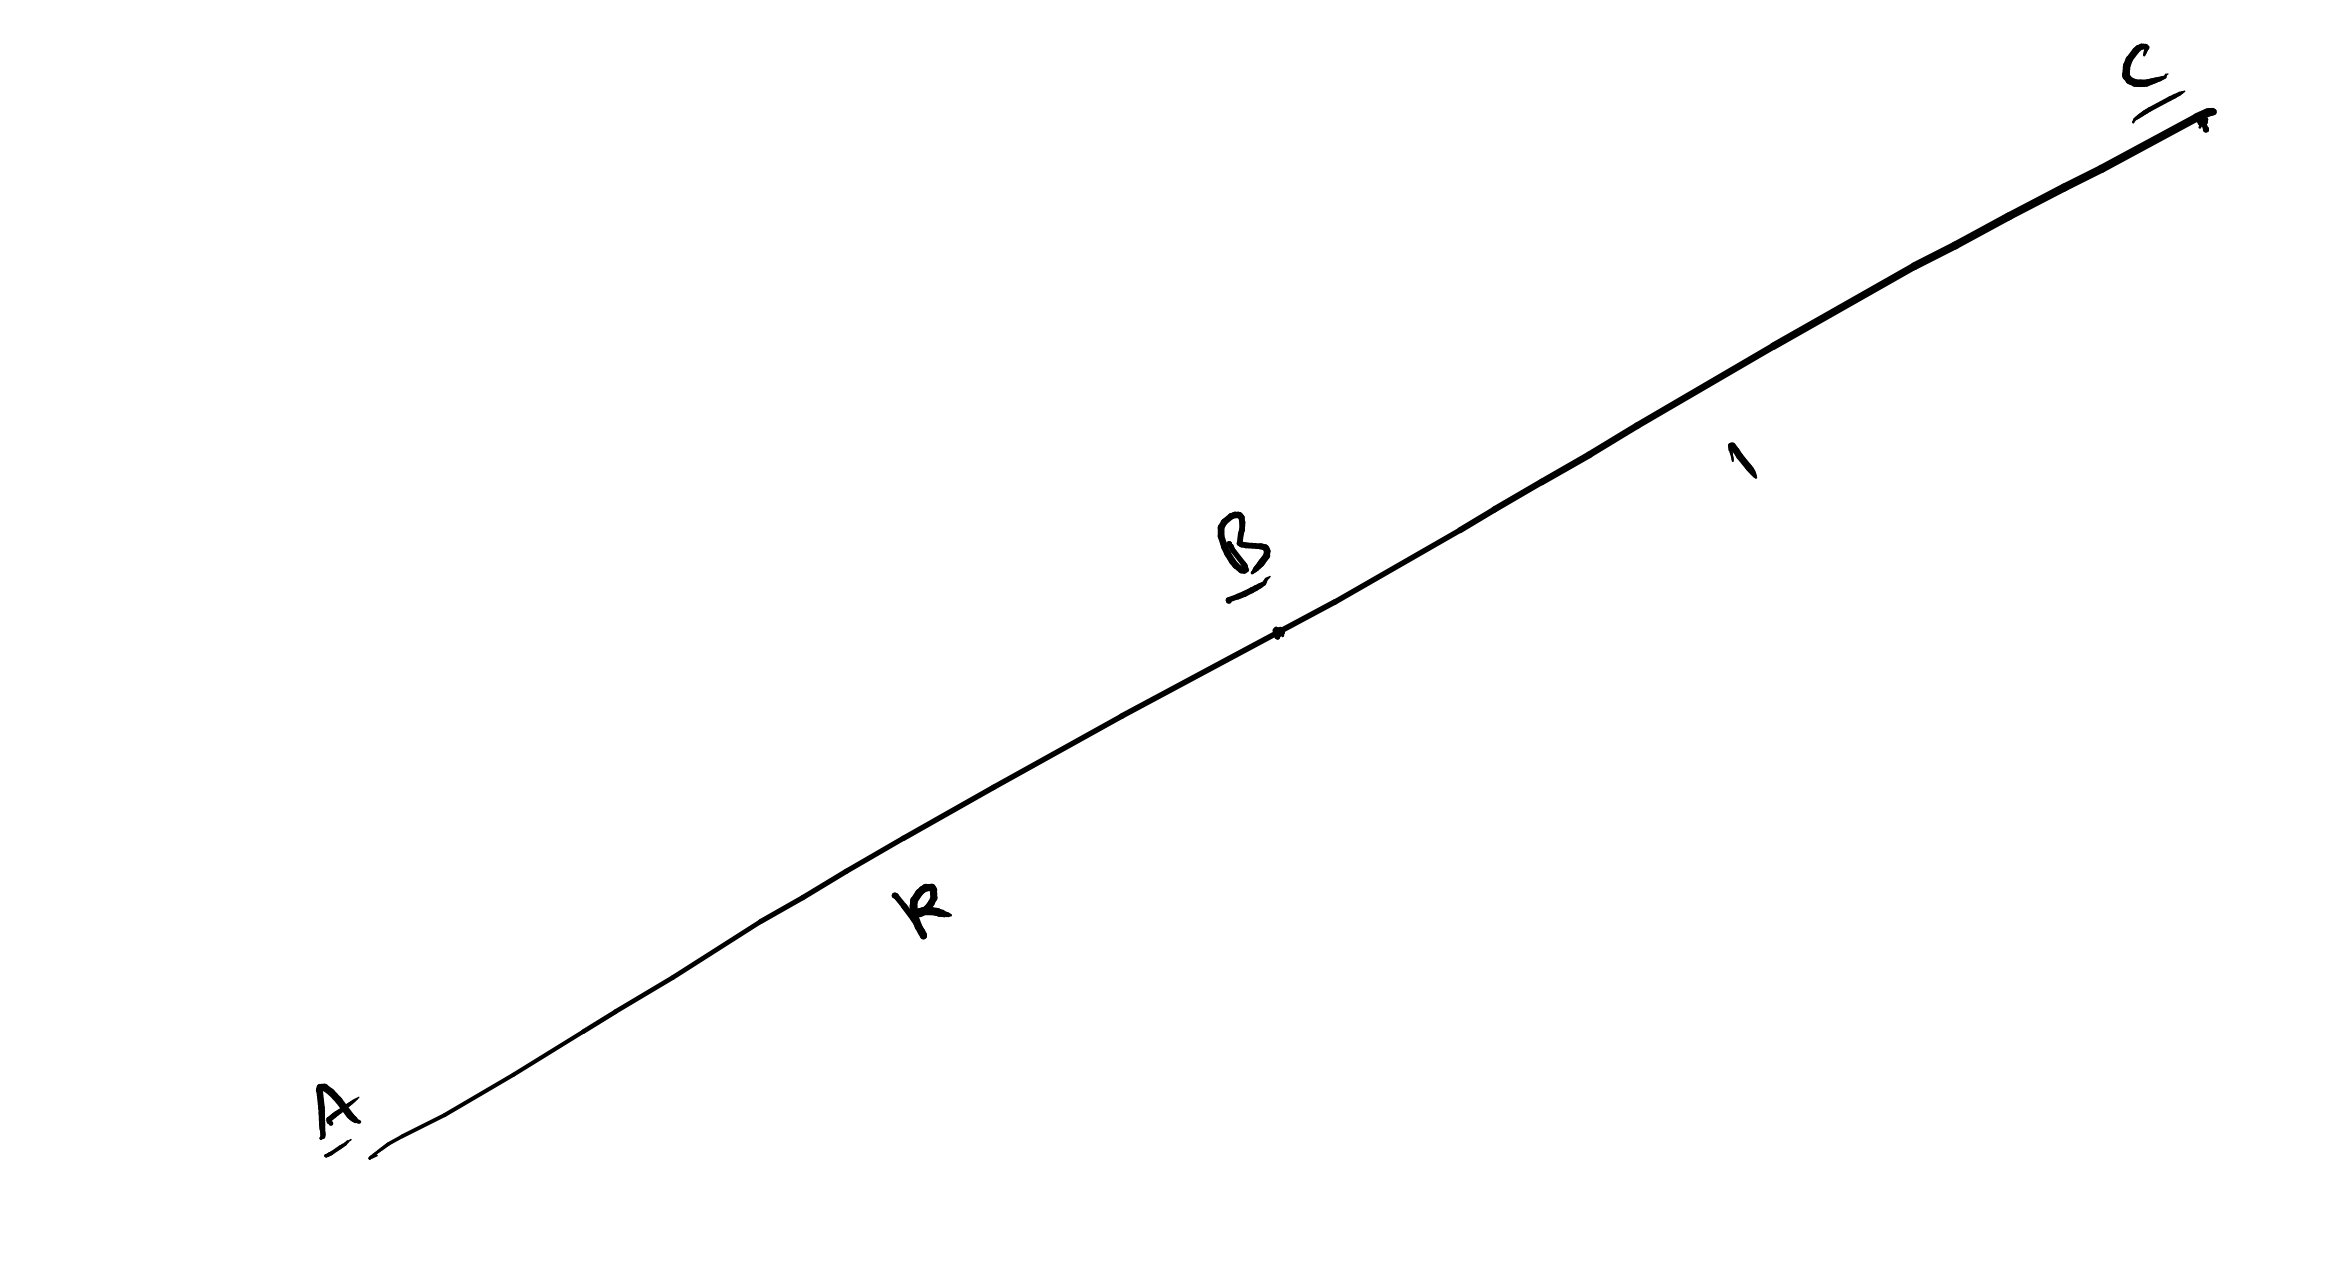
\includegraphics[width=\columnwidth]{./figs/ratio.eps}
\caption{}
\label{fig:ratio}
\end{figure}
\solution From \eqref{eq:nhomog}, 
\begin{align}
\begin{split}
\vec{B} &= \vec{A} + \lambda_1 \myvec{1 \\ m},
\\
\vec{B} &= \vec{C} - \lambda_2 \myvec{1 \\ m}.
\end{split}
\\
\label{eq:rat_1}
\implies \frac{\norm{\vec{A}-\vec{B}}}{\norm{\vec{B}-\vec{C}}} &= 
\frac{\lambda_1}{\lambda_2} = k
\\
\text{and } \frac{\vec{B}- \vec{A}}{\lambda_1} &= \frac{\vec{C}- 
\vec{B}}{\lambda_2} =  \myvec{1 \\ m},
\label{eq:rat_2}
\end{align}
%
from \eqref{eq:k}. Using \eqref{eq:rat_1} and \eqref{eq:rat_1},
\begin{align}
\vec{A}- \vec{B} &=  k\brak{\vec{B}- \vec{C}}
\end{align}
%
resulting in \eqref{eq:ratio}.
%
\item If $\vec{A}$ and $\vec{B}$ are linearly independent,  
\begin{equation}
k_1\vec{A} + k_2\vec{B} = 0 \implies k_1=k_2=0
\end{equation}
\item $BE$ and $CF$ are medians of $\triangle ABC$ intersecting at $O$ as shown in Fig. \ref{fig:median}. 
Show that
\begin{equation}
\frac{CO}{OF} = \frac{BO}{OE} = 2
\end{equation}
%
\begin{figure}[!hb]
\centering
\includegraphics[width=\columnwidth]{./figs/median.eps}
\caption{}
\label{fig:median}
\end{figure}
\solution Let
\begin{align}
\frac{CO}{OF} &= k_1
\\
\frac{BO}{OE} &= k_2
\end{align}
%
Using  \eqref{eq:ratio},
\begin{align}
\vec{E}&= \frac{\vec{A} + \vec{C}}{2}
\\
\vec{F}&= \frac{\vec{A} + \vec{B}}{2}
\end{align}
%
and
\begin{align}
\label{eq:o1}
\vec{O}&= \frac{k_1\vec{F} + \vec{C}}{k_1+1} = \frac{k_1\frac{\vec{A} + \vec{B}}{2} + \vec{C}}{k_1+1}
\\
\vec{O}&= \frac{k_2\vec{E} + \vec{B}}{k_2+1} = \frac{k_2\frac{\vec{A} + \vec{C}}{2} + \vec{B}}{k_2+1}
\label{eq:o2}
\end{align}
%
From \eqref{eq:o1} and \eqref{eq:o2},
\begin{align}
 \frac{k_1\frac{\vec{A} + \vec{B}}{2} + \vec{C}}{k_1+1} &= 
 \frac{k_2\frac{\vec{A} + \vec{C}}{2} + \vec{B}}{k_2+1}
\end{align}
\begin{multline}
\label{eq:lin_comb}
\implies \sbrak{\frac{k_1\brak{k_2+1}}{2}
-\frac{k_2\brak{k_1+1}}{2}}\vec{A} 
\\
+ 
\sbrak{\frac{k_1\brak{k_2+1}}{2}-\brak{k_1+1}}\vec{B} 
\\
+ \sbrak{\brak{k_2+1}-\frac{k_2\brak{k_1+1}}{2}}\vec{C} 
= 0
\end{multline}
resulting in $k_1 = k_2$,
\begin{align}
k_1^2-k_1-2  &= 0
\implies k_1 = k_2 = 2,
\end{align}
provided $\vec{A},\vec{B},\vec{C}$ are linearly independent. Thus, substituting $k_1=2$ in \eqref{eq:o2},
\begin{equation}
\vec{O} = \frac{\vec{A}+\vec{B}+\vec{C}}{3}
\end{equation}
%
If $\vec{A},\vec{B},\vec{C}$ are linearly dependent,
\begin{align}
\label{eq:lin_dep}
\vec{A} = \alpha \vec{B} + \beta \vec{C} 
\end{align}
%
Note that $\vec{B},\vec{C}$ are linearly independent.
Substituting \eqref{eq:lin_dep} in \eqref{eq:lin_comb},
\begin{multline}
%\label{eq:lin_comb}
 \sbrak{\frac{k_1\brak{k_2+1}}{2}
-\frac{k_2\brak{k_1+1}}{2}}\sbrak{\alpha \vec{B} + \beta \vec{C}  }
\\
+ 
\sbrak{\frac{k_1\brak{k_2+1}}{2}-\brak{k_1+1}}\vec{B} 
\\
+ \sbrak{\brak{k_2+1}-\frac{k_2\brak{k_1+1}}{2}}\vec{C} 
= 0
\end{multline}
\begin{align}
\implies
\begin{split}
\brak{k_1-k_2}\alpha + k_1k_2 - k_1-2 &=0
\\
\brak{k_1-k_2}\beta - k_1k_2 + k_2+2 &=0
\end{split}
\label{eq:median_contra}
\\
\implies \brak{k_1-k_2}\brak{\alpha +\beta - 1} = 0
\end{align}
If $\alpha+\beta = 1, \vec{A},\vec{B},\vec{C}$ are collinear according to \eqref{eq:ratio} resulting in a 
contradiction.  Hence, $k_1=k_2$, which, upon substitution in \eqref{eq:median_contra}, yields
\begin{equation}
k_1^2 - k_1-2 = 0 \implies k_1 = 2.
\end{equation}
\end{enumerate}
%
\end{document}
